\documentclass{standalone}
\usepackage{tikz}
% put any importmodules into the preamble
\begin{document}
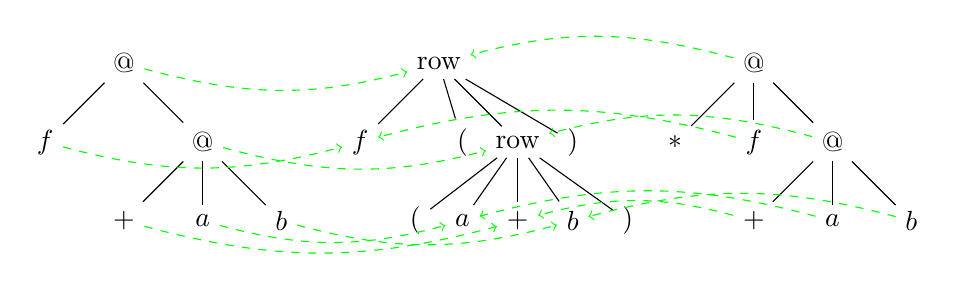
\begin{tikzpicture} 
% presentation tree
\node (p1f) at (0,1) {$f$};
\node (p1a1) at (1,2) {row};
\node (p1a2o) at (1.3,1) {$($};
\node (p1a2) at (2,1) {row};
\node (p1a2c) at (2.7,1) {$)$};
\node (p1o) at (.7,0) {$($};
\node (p1a) at (1.3,0) {$a$};
\node (p1p) at (2,0) {$+$};
\node (p1b) at (2.7,0) {$b$};
\node (p1c) at (3.4,0) {$)$};
\draw (p1a1) -- (p1f);
\draw (p1a1) -- (p1a2o);
\draw (p1a1) -- (p1a2);
\draw (p1a1) -- (p1a2c);
\draw (p1a2) -- (p1p);
\draw (p1a2) -- (p1a);
\draw (p1a2) -- (p1b);
\draw (p1a2) -- (p1o);
\draw (p1a2) -- (p1c);
% product 
\node (c1a1) at (5,2) {$@$};
\node (c1t) at (4,1) {$*$};
\node (c1f) at (5,1) {$f$};
\node (c1a2) at (6,1) {$@$};
\node (c1p) at (5,0) {$+$};
\node (c1a) at (6,0) {$a$};
\node (c1b) at (7,0) {$b$};
\draw (c1a1) -- (c1f);
\draw (c1a1) -- (c1t);
\draw (c1a1) -- (c1a2);
\draw (c1a2) -- (c1p);
\draw (c1a2) -- (c1a);
\draw (c1a2) -- (c1b);
\draw[->,green,dashed] (c1f) to[out=165,in=15] (p1f);
\draw[->,green,dashed] (c1a1) to[out=165,in=15] (p1a1);
\draw[->,green,dashed] (c1a2) to[out=165,in=15] (p1a2);
\draw[->,green,dashed] (c1p) to[out=165,in=15] (p1p);
\draw[->,green,dashed] (c1a) to[out=165,in=15] (p1a);
\draw[->,green,dashed] (c1b) to[out=165,in=15] (p1b);

% application
\node (c2f) at (-4,1) {$f$};
\node (c2a1) at (-3,2) {$@$};
\node (c2a2) at (-2,1) {$@$};
\node (c2p) at (-3,0) {$+$};
\node (c2a) at (-2,0) {$a$};
\node (c2b) at (-1,0) {$b$};
\draw (c2a1) -- (c2f);
\draw (c2a1) -- (c2a2);
\draw (c2a2) -- (c2p);
\draw (c2a2) -- (c2a);
\draw (c2a2) -- (c2b);
\draw[->,green,dashed] (c2f) to[out=-15,in=195] (p1f);
\draw[->,green,dashed] (c2a1) to[out=-15,in=195] (p1a1);
\draw[->,green,dashed] (c2a2) to[out=-15,in=195] (p1a2);
\draw[->,green,dashed] (c2p) to[out=-15,in=195] (p1p);
\draw[->,green,dashed] (c2a) to[out=-15,in=195] (p1a);
\draw[->,green,dashed] (c2b) to[out=-15,in=195] (p1b);
\end{tikzpicture}
\end{document}
%%% Local Variables: 
%%% mode: latex
%%% TeX-master: t
%%% End: 

% LocalWords:  tikzpicture
